\documentclass[10pt]{article}
% generated by Madoko, version 1.2.0
%mdk-data-line={1}


\usepackage[heading-base={2},section-num={False},bib-label={hide},fontspec={True}]{madoko2}


\begin{document}



%mdk-data-line={30}
\mdxtitleblockstart{}
%mdk-data-line={30}
\mdxtitle{\mdline{30}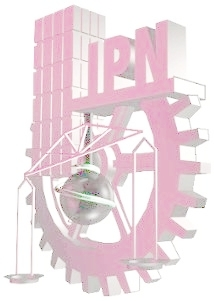
\includegraphics[keepaspectratio=true,width=\dimwidth{0.10}]{images/poli}{} IPN-UPIITA}%mdk

%mdk-data-line={33}
\mdxsubtitle{\mdline{33}Redes Neuronales}%mdk

%mdk-data-line={36}
\mdxtitlenote{\mdline{36}Reporte R02}%mdk
\mdxauthorstart{}
%mdk-data-line={41}
\mdxauthorname{\mdline{41}Dr. Rafael Martínez Martínez}%mdk

%mdk-data-line={44}
\mdxauthoraddress{\mdline{44}Academia de sistemas}%mdk

%mdk-data-line={47}
\mdxauthoremail{\mdline{47}ramartinezr@ipn.mx}%mdk
\mdxauthorend\mdtitleauthorrunning{}{}\mdxtitleblockend%mdk

%mdk-data-line={33}
\mdhr{}%mdk

%mdk-data-line={34}
\begin{mddefinitions}%mdk

\mddefterm{\noindent{\bfseries Instrucciones:}}%mdk

%mdk-data-line={34}
\begin{mdbmarginx}{}{}{}{1.5em}%mdk
\begin{mddefdata}%mdk

%mdk-data-line={34}
\begin{itemize}[noitemsep,topsep=\mdcompacttopsep]%mdk

%mdk-data-line={34}
\item\mdline{34}Cada problema/ejercicio debe tener procedimiento ordenado y completo que justifique adecuadamente la respuesta anotada. \mdline{34}\mdline{34}%mdk
%mdk
\end{itemize}%mdk
%mdk
\end{mddefdata}%mdk
\end{mdbmarginx}%mdk

%mdk-data-line={36}
\begin{mdbmarginx}{}{}{}{1.5em}%mdk
\begin{mddefdata}%mdk

%mdk-data-line={36}
\begin{itemize}[noitemsep,topsep=\mdcompacttopsep]%mdk

%mdk-data-line={36}
\item\mdline{36}Si falta el procedimiento o este no justifica la respuesta anotada entonces el problema vale 0 puntos aunque la respuesta sea correcta.%mdk
%mdk
\end{itemize}%mdk
%mdk
\end{mddefdata}%mdk
\end{mdbmarginx}%mdk
%mdk
\end{mddefinitions}%mdk

%mdk-data-line={37}
\mdhr{}%mdk
\mdline{38}
\begin{mdtoc}%mdk

\section*{Contenido}\label{sec-contenido}%mdk%mdk

\begin{mdtocblock}%mdk

\mdtocitemx{sec-problema-1-50-puntos}{\mdref{sec-problema-1-50-puntos}{Problema 1 (50 puntos)}}%mdk

\mdtocitemx{sec-problema-2-50-puntos}{\mdref{sec-problema-2-50-puntos}{Problema 2 (50 puntos)}}%mdk
%mdk
\end{mdtocblock}%mdk
%mdk
\end{mdtoc}%mdk

%mdk-data-line={40}
\section*{\mdline{40}Problema 1 (50 puntos)}\label{sec-problema-1-50-puntos}%mdk%mdk

%mdk-data-line={42}
\begin{quote}%mdk

%mdk-data-line={42}
\noindent\mdline{42}Walter Pitts salio de las calles al MIT, pero no pudo escapar de sí mismo. \mdline{42}\mdbr
\mdline{43}\hspace*{1em}\mdline{43}%mdk

%mdk-data-line={45}
\mdline{45} La vida de Walter Pitts pasó de un vagabundo fugitivo, a pionero de la neurociencia del MIT, a alcohólico retraído.%mdk
%mdk
\end{quote}%mdk

%mdk-data-line={48}
\noindent\mdline{48}En 1943 Warren McCulloch y Walter Pitts introdujeron una de las primeras neuronas artificiales. La referencia de dicho trabajo es la siguiente:%mdk

%mdk-data-line={50}
\mdline{50}\emph{W. McCulloch and W. Pitts, “A logical calculus of the ideas immanent in nervous activity,” Bulletin of Mathematical Biophysics, Vol. 5, pp. 115–133, 1943.}\mdline{50}%mdk

%mdk-data-line={52}
\mdline{52}Este articulo introduce el primer modelo matemático de una neurona, en la cual la suma ponderada de las señales de entrada es comparada con un umbral que determina la salida de la neurona. Cuando la suma es más grande o igual al umbral, la salida es \mdline{52}$1$\mdline{52}. Cuando la suma es menor al umbral, la salida es \mdline{52}$0$\mdline{52}. A diferencia de las redes biológicas, los parámetros de su red (pesos) se tenían que diseñar y no proporcionaron un método de entrenamiento. Sin embargo, fue el precedente sobre un campo interesante entre la conexión de la biología y las computadoras digitales.%mdk

%mdk-data-line={54}
\mdline{54}A finales de la década de los 50\mdline{54}`\mdline{54}s del siglo pasado, Frank Rosenblatt y otros investigadores desarrollaron una clase de redes neuronales llamada perceptrones:%mdk

%mdk-data-line={56}
\mdline{56}\emph{F. Rosenblatt, “The perceptron: A probabilistic model for information storage and organization in the brain,” Psycho- logical Review, Vol. 65, pp. 386–408, 1958.}\mdline{56}%mdk

%mdk-data-line={58}
\mdline{58}Su modelo era parecido al de McCulloch y Pitts, pero además proponían una regla de aprendizaje para resolver el problema de reconocimiento de patrones. Posteriormente se mostró que este aprendizaje estaba limitado a resolver problemas de reconocimiento linealmente separables. Y no fue hasta la década de los 80\mdline{58}`\mdline{58}s del siglo pasado, que esta limitación se resolvió utilizando múltiples capas de perceptrones.%mdk

%mdk-data-line={60}
\mdline{60}La colaboración de Warren McCulloch y Walter Pitts va más allá de la profesional. 
En el artículo de divulgación\mdline{61}~\href{https://nautil.us/issue/21/information/the-man-who-tried-to-redeem-the-world-with-logic}{The Man Who Tried to Redeem the World with Logic}\mdline{61}, 
se resume un poco de la desgarradora vida de Pitts. En la lectura se podrá observar como Pitts 
colaboró con algunas de las grandes mentes del siglo XX. Para este problema es necesario realizar 
la lectura del articulo de divulgación mencionado. Para el control de dicha lectura, se responden 
las siguientes preguntas (lo principal es tu reflexión, que no se pide, sobre el contenido de la lectura):%mdk

%mdk-data-line={68}
\begin{enumerate}[noitemsep,topsep=\mdcompacttopsep]%mdk

%mdk-data-line={68}
\item\mdline{68}¿Qué edad tenia Pitts cuando le escribió a  Bertrand Russell sobre los errores en su libro?%mdk

%mdk-data-line={69}
\item\mdline{69}¿Quién presento a Pitts con McCulloch?%mdk

%mdk-data-line={70}
\item\mdline{70}¿Quienes conformaban el núcleo del grupo conocido como \mdline{70}\emph{los cibernéticos}\mdline{70}?%mdk

%mdk-data-line={71}
\item\mdline{71}¿Cuál fue el motivo por el cual Norbert Wiener dejo de tener comunicación con Pitts?%mdk

%mdk-data-line={72}
\item\mdline{72}¿Cuáles fueron los eventos que llevaron a Pitts a hundirse en depresión, y quemar su tesis doctoral y sus escritos?%mdk

%mdk-data-line={73}
\item\mdline{73}¿Consideras que si Pitts hubiera tenido una situación diferente a la que tuvo en el lugar donde nacio, podría haber superado los eventos que lo llevaron a la depresión? Explica%mdk
%mdk
\end{enumerate}%mdk

%mdk-data-line={81}
\section*{\mdline{81}Problema 2 (50 puntos)}\label{sec-problema-2-50-puntos}%mdk%mdk

%mdk-data-line={83}
\noindent\mdline{83}La siguiente\mdline{83}~\href{http://playground.tensorflow.org/\%23activation=tanh\%26batchSize=10\%26dataset=circle\%26regDataset=reg-plane\%26learningRate=0.03\%26regularizationRate=0\%26noise=0\%26networkShape=4,2\%26seed=0.12132\%26showTestData=false\%26discretize=false\%26percTrainData=50\%26x=true\%26y=true\%26xTimesY=false\%26xSquared=false\%26ySquared=false\%26cosX=false\%26sinX=false\%26cosY=false\%26sinY=false\%26collectStats=false\%26problem=classification\%26initZero=false\%26hideText=false}{aplicación web}\mdline{83}, permite elegir gráficamene una topologia de red (feedforward) para resolver problemas de
clasificación y regresión prestablecidos.%mdk

%mdk-data-line={86}
\mdline{86}La Figura\mdline{86}~\mdref{fig-play}{\mdcaptionlabel{1}}\mdline{86} muestra la elección de una topología para resolver un problema (porporcionado en la aplicación) de clasificación. 
Se han elegido algunas capas ocultas\mdline{87}\mdfootnote{1}{%mdk-data-line={129}
%mdk-data-line={129}
\noindent\mdline{129}Por el momento pensemos que si se tiene más de una capa, el entrenamiento se lleva acabo de alguna manera, que por el momento no nos importa especificar.%mdk
\label{fn-capas}%mdk%mdk
}\mdline{87} y los demás parámetros de la red. 
Al comenzar en entrenamiento y deternerlo después de 143 epocas, los valores de los pesos
se pueden consultar colocando el puntero sobre las lineas de cada capa.\mdline{89} \mdline{89}%mdk

%mdk-data-line={91}
\begin{figure}[tbp]%mdk
\begin{mdcenter}%mdk

%mdk-data-line={92}
\noindent\mdline{92} \mdline{92}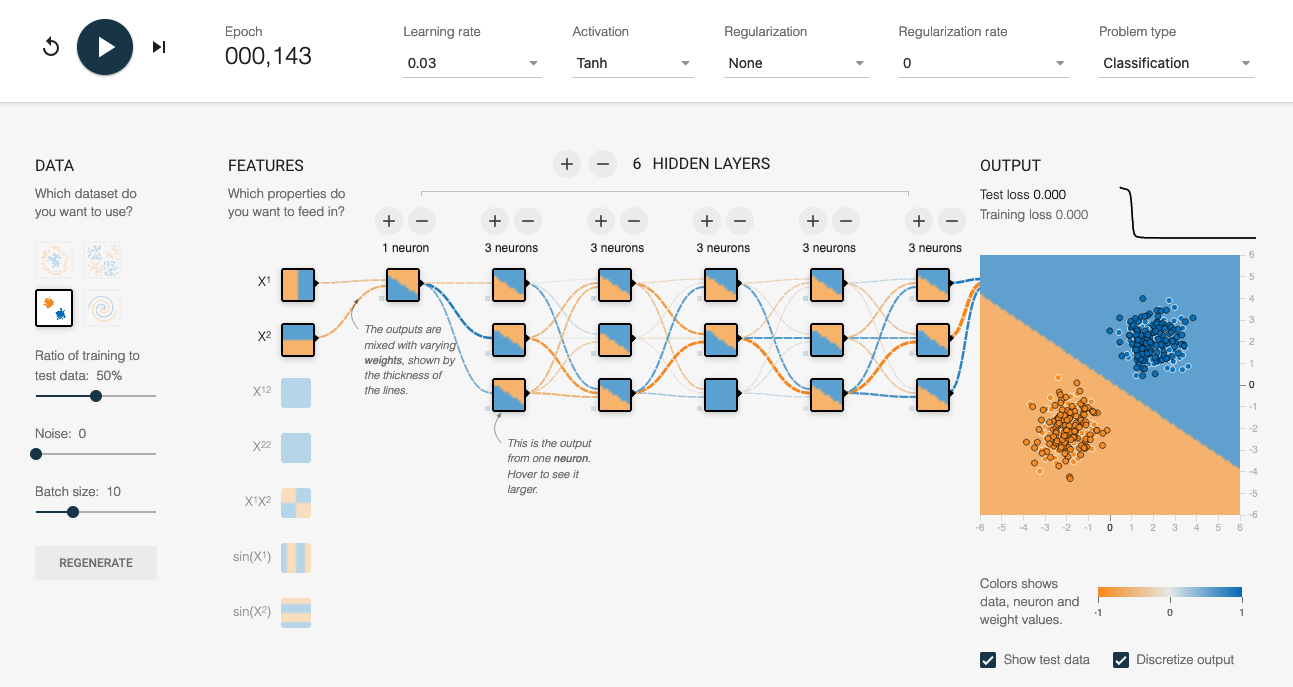
\includegraphics[keepaspectratio=true,width=\dimwidth{1.00}]{images/playground}{}\mdline{92}%mdk

%mdk-data-line={93}
\mdhr{}%mdk

%mdk-data-line={94}
\noindent\mdline{94}\mdcaption{\textbf{Figura~\mdcaptionlabel{1}.}~\mdcaptiontext{Red elegida par resolver el problema de clasificación indicado}}%mdk
%mdk
\end{mdcenter}\label{fig-play}%mdk
%mdk
\end{figure}%mdk

%mdk-data-line={95}
\mdline{95}Si bien se tienen dos entradas en cada problema de clasificación (en esta aplicación), la aplicación nos permite generar 5 entradas adicionales construidas con
los dos datos de entrada, además tiene la opción de tomar estas entras \mdline{96}\emph{artificiales}\mdline{96} como información adicional para entrenar la red. 
Es decir, se puede pensar que dado un problema con \mdline{97}$m$\mdline{97} entradas se puede transformar a un problema de \mdline{97}$n+m$\mdline{97} entradas, donde \mdline{97}$n$\mdline{97} 
es el número de datos construidos \mdline{98}\emph{artificialmente}\mdline{98} transformando los \mdline{98}$m$\mdline{98} datos iniciales. En el caso de la aplicación \mdline{98}$n=5$\mdline{98}.%mdk

%mdk-data-line={100}
\mdline{100}Conteste las siguiente preguntas%mdk

%mdk-data-line={102}
\begin{enumerate}%mdk

%mdk-data-line={102}
\item{}
%mdk-data-line={102}
\mdline{102}¿A qué se refiere que una red sea feedforward?%mdk%mdk

%mdk-data-line={103}
\item{}
%mdk-data-line={103}
\mdline{103}¿Cuantos problemas de clasificación y cuantos de regresión tiene prestablecidos la aplicación?%mdk%mdk

%mdk-data-line={104}
\item{}
%mdk-data-line={104}
\mdline{104}Investiga a que se refieren los siguientes elementos que aparecen en la aplicación\mdline{104}\mdfootnote{2}{%mdk-data-line={130}
%mdk-data-line={130}
\noindent\mdline{130}Explicación breve, si lo consideras necesario anota ecuaciónes como ejemplo%mdk
\label{fn-np}%mdk%mdk
}\mdline{104}:%mdk

%mdk-data-line={105}
\begin{enumerate}[noitemsep,topsep=\mdcompacttopsep,label=\alph*.]%mdk

%mdk-data-line={105}
\item\mdline{105}Learning rate%mdk

%mdk-data-line={106}
\item\mdline{106}Regularization%mdk

%mdk-data-line={107}
\item\mdline{107}Regularization rate%mdk

%mdk-data-line={108}
\item\mdline{108}Radio of training to test data%mdk

%mdk-data-line={109}
\item\mdline{109}Batch size%mdk

%mdk-data-line={110}
\item\mdline{110}Test loss%mdk

%mdk-data-line={111}
\item\mdline{111}Training loss%mdk
%mdk
\end{enumerate}%mdk%mdk

%mdk-data-line={112}
\item{}
%mdk-data-line={112}
\mdline{112}Es claro que la topologia elegida en la Figura\mdline{112}~\mdref{fig-play}{\mdcaptionlabel{1}}\mdline{112} \mdline{112}\emph{está sobrada}\mdline{112}. Pues tenemos un problema de clasificación 
linealmente separable. Resuelve este problema con una capa, una neurona, las dos estradas \mdline{113}\emph{naturales}\mdline{113},
y la elección de tu preferencia de los demás 
parámetros (función de activación, Learnin rate, etc.), no es necesario justificar la elección de los parámetros.%mdk

%mdk-data-line={116}
\begin{enumerate}[noitemsep,topsep=\mdcompacttopsep,label=\alph*.]%mdk

%mdk-data-line={116}
\item\mdline{116}Solo reporta la imagen correspondiente, donde se pueda apreciar 
que se llevó acabo el entrenamiento de forma exitosa.%mdk

%mdk-data-line={118}
\item\mdline{118}¿Cuántas epocas de entrenamiento fueron necesarias (para esto utiliza el boton a un costado de \mdline{118}\emph{play}\mdline{118})?%mdk
%mdk
\end{enumerate}%mdk%mdk

%mdk-data-line={119}
\item{}
%mdk-data-line={119}
\mdline{119}\textbf{Juega con la aplicación}\mdline{119}. Resuelve los problemas de clasificación restantes, utilizando la menor cantidad de capas posibles y
la menor cantidad de neuronas posibles en cada capa\mdline{120}\mdfootnote{3}{%mdk-data-line={131}
%mdk-data-line={131}
\noindent\mdline{131}Varias topologias resolverán el problema, queremos la más secilla que puedas construir, en este caso nos referimos a sencilla en el sentido de minimizar el numero de capas y neuronas%mdk
\label{fn-sen}%mdk%mdk
}\mdline{120}.
Todos los demás parámetros se pueden elegir a tu consideración 
(entradas, función de activación, Learnin rate, etc.) no es necesario justificar la elección de los parámetros.
Reporta solo las imagenes correspondientes, donde se pueda apreciar 
que se llevó acabo el entrenamiento de forma exitosa.%mdk%mdk
%mdk
\end{enumerate}%mdk%mdk


\end{document}
